%*******************************************************************************
%*********************************** Chapter XXXXXXXX *****************************
%*******************************************************************************

\chapter{Simulations of the DUNE Far Detector}  %Title of chapter
\graphicspath{{FarDetectorSimulations/Figs/Raster/}{FarDetectorSimulations/Figs/PDF/}{FarDetectorSimulations/Figs/}}

Previous work presented has been done concerning the 35 ton prototype, however it is also important to simulate the DUNE Far Detector (FD). Simulations in the FD have concentrated on cosmogenic background to neutrino oscillations, in Section~\ref{sec:LBNESurf}, and the muon background to nucleon decay, in Section~\ref{sec:DUNENDK}. The simulations shown in Section~\ref{sec:LBNESurf} are discussed in!!!!~citep{MartinsThesis}!!!!, and were performed for the Long Baseline Neutrino Experiment (LBNE) which along with the Long Baseline Neutrino Oscillation (LBNO) experiment formed the basis for DUNE and so are included here for completeness. The other work presented was performed for the DUNE collaboration in conjunction with work done by Vitaly Kudryavtsev and Matthew Robinson, both of the University of Sheffield, and was performed with the aim of producing muon-induced background limits to nucleon decay. \\

%********************************** %Second Section  **************************************
\section{Simulations of the LBNE surface detector} \label{sec:LBNESurf} %Section - X.2

%********************************** % Third Section  *************************************
\section{The use of MUSUN in LArSoft} \label{sec:FDIncorporation}  %Section - X.3
The primary muons in the following discussions are all generated using MUSIC~\citep{MUSUN}~\citep{MUSIC}~\citep{MUSIC2} and MUSUN~\citep{MUSUN}~\citep{MUSUN2}, and so a brief overview of them is required. MUSIC first propogates muons through a medium defined by the user for given initial energies, positions and direction cosines. A range of energies between 10$^2$ and 10$^7$ GeV are considered and their energy distributions are stored at depths of between 100 and 15,000 m w.e. Energy losses due to four processes are considered; ionisation, bremsstrahlung, electron-positron pair production and muon-nucleus inelastic scattering. The output of MUSIC is then used by MUSUN to generate a muon energy spectrum and angular distribution for a given detector location given details about the local surface profile. \\

The location of the DUNE detector near the Ross shaft at SURF has global coordinates of: latitude = 44$^{\circ|}$20$'$45.21$''$ N and longitude 103$^{\circ}$45$'$16.13$''$ West. The rock composition is assumed to be $< Z >$ = 12.09 and $< A >$ = 24.17, and the density is assumed to be 2.70 g cm${-3}$~\citep{Mei:2009py}. The flux calculated by MUSIC/MUSUN of 5.18 $\times$ 10$^{-9}$ cm$^{-2}$ s$^{-1}$ sr$^{-1}$ is well matched to the flux measured by the active veto system of the Davis' experiment which was (5.38 $\pm$ 0.07) $\times$ 10$^{-9}$ cm$^{-2}$ s$^{-1}$ sr$^{-1}$~\citep{PhysRevD.27.1444}. Given small differences in these values and another measurement by the Majorana demonstator, the systematic uncertainty in calculating the muon flux is estimated to be 20\%~\citep{NDKTFNote}. \\

The surface profile around the proposed detector location is shown in Figure~\ref{fig:SurfProf_Col}, where the proposed location is in the centre of the map. Each quadrant on the map has been divided into 4 angles of 22$^{\circ}$ to help quide the eye when comparing to Figure~\ref{fig:SurfProf_Azi}, where the distribution of azimuth angles is plotted. The vertical lines in Figure~\ref{fig:SurfProf_Azi} show the division of the quadrants when the angle is calcualted from East. When moving from East to North it is possible to discern how the peaks and troughs on the surface profile correspond to troughs and peaks in the distribution of azimuthal angle. \\

\begin{figure}[h!]
  \centering
  \begin{subfigure}{0.45\textwidth}
    \centering
    \includegraphics[width=\textwidth]{dune-surface-map}
    \caption{The surface profile of the DUNE far detector site at SURF.}
    \label{fig:SurfProf_Col}
  \end{subfigure}
  \hspace{0.08\textwidth}
  \begin{subfigure}{0.45\textwidth}
    \centering
    \includegraphics[width=\textwidth]{phi-map}
    \caption{The distribution of azimuthal angles of muons at the DUNE far detector site at SURF.}
    \label{fig:SurfProf_Azi}
  \end{subfigure}
  \caption[The correlation between the surface profile and distribution of azimuthal angles at the DUNE far detector site]
          {The correlation between the surface profile and distribution of azimuthal angles at the DUNE far detector site. The quadrants have been divided into four angles of equal size. The azimuthal angle, calculated as the angle from East (pointing to the right in Fig.~\ref{fig:SurfProf_Col}), and increasing counterclockwise, is seen to follow the contours of the surface profile.}
\end{figure}

Given these parameters the muon flux when assuming a spherical detector geometry without simulating a detector cavern is given by Table~\ref{tab:MUSUNflux}. \\
\begin{table}[h!]
\caption[Muon flux parameters as calculated with MUSIC/MUSUN.]
        {Muon flux parameters as calculated with MUSIC/MUSUN.}
\centering
\label{tab:MUSUNflux}
\begin{tabular}{c c c c}
\toprule
{Total flux (cm$^{-2}$ s$^{-1}$)} & {Mean E$_{\mu}$ (GeV)} & {Mean slant depth (m w.e)} & {Mean $\theta$ ($^{\circ}$)} \\ 
\midrule
5.66 $\times$ 10$^{-9}$           & 283                    & 4532                       & 26                           \\
\bottomrule
\end{tabular}
\end{table}

The muons simulated for DUNE are sampled on a the surface of a box surrounding the detector hall that also encompassed 7 m of rock above the cavern, and 5 m of rock on all other sides. This is to ensure that there is sufficient rock to induce cascades both above and around the detector hall, as it is mainly the secondaries produced in these interactions that enter the detector which are of concern to nucleon decay searches. This will be discussed in Section~\ref{sec:DUNENDK}. The size of the box the muons are sampled from is 74.43 $\times$ 29.54 $\times$ 30.18 m$^3$, compared to the simulated cryostat that has dimensions of 61.62 $\times$ 14.94 $\times$ 13.58 m$^3$, where these dimensions are (length $\times$ width $\times$ height). The muons are sampled randomly according to their energy spectrum for a given zenith and azimuthal angle, using the angular distribution obtained with MUSIC. \\

Before this could be done however, MUSUN had to be incorporated into the DUNE software framework as it has previously been maintained in FORTRAN as an external package. This involved building on the work done by the LZ collaboration in porting the code to C++~!!!!!citep{Kareem}. The process by which this was done was to first reproduce the distributions produced by the LZ collaboration with the DUNE software framework using the LZ detector location, and then reproducing the muon distributions produced by the original FORTRAN code for the DUNE detector location. The dsitributions produced by the DUNE software framework are shown in Figure~\ref{fig:MUSUNIncorp}, these are seen to be consistent with the same distributions shown in~\citep{MUSUNLBNE}. The initial positions of 10,000 muons generated in LArSoft around the DUNE 10 kt module that is simulated is shown in Figure~\ref{fig:10ktPos}. The initial positions of the muons are shown as blue points, whilst the cryostat is a single black box and each TPC is a single red box. \\

\begin{figure}[h!]
  \centering
  \begin{subfigure}{0.45\textwidth}
    \centering
    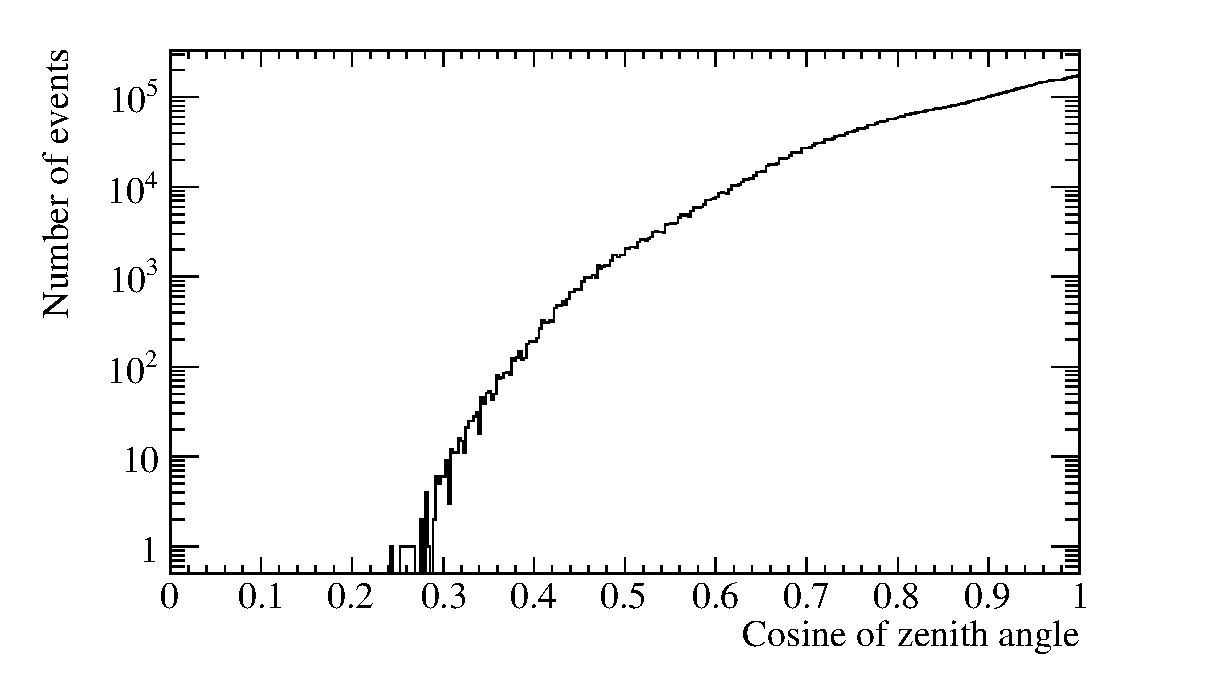
\includegraphics[width=\textwidth]{ZenithCan}
    \caption{Distribution of zenith angles.}
  \end{subfigure}
  \hspace{0.08\textwidth}
  \begin{subfigure}{0.45\textwidth}
    \centering
    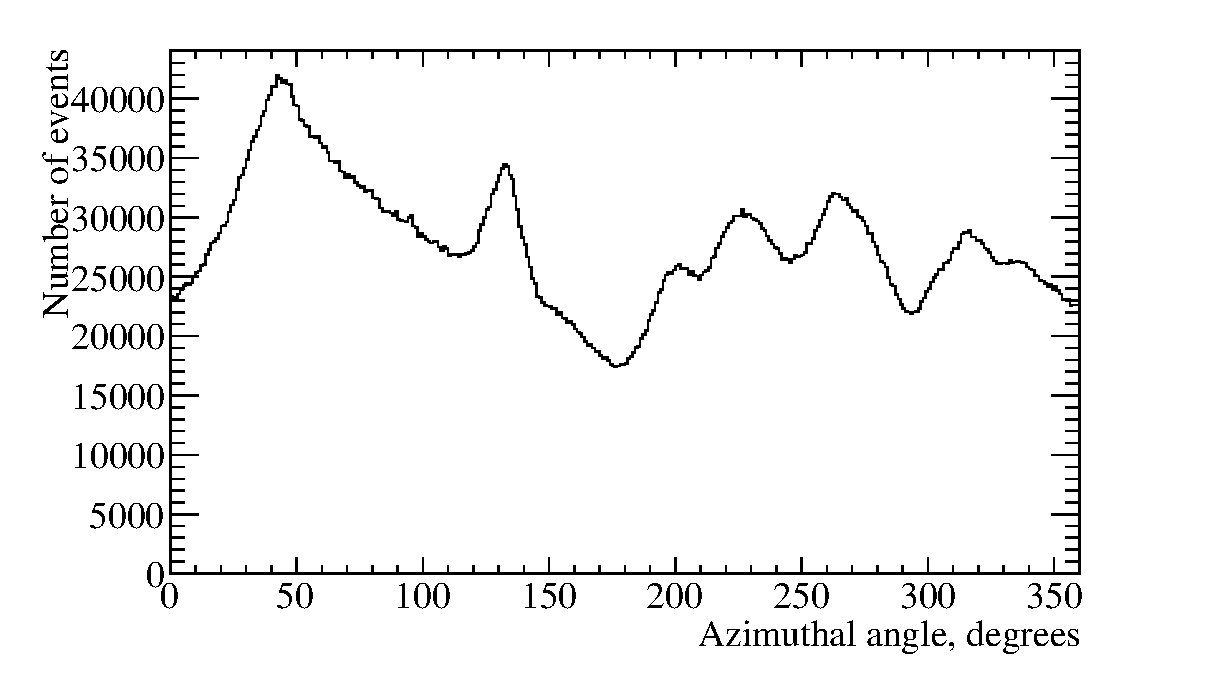
\includegraphics[width=\textwidth]{AzimuthCan}
    \caption{Distribution of azimuthal angles.}
  \end{subfigure}
  % ========
  \begin{subfigure}{0.45\textwidth}
    \centering
    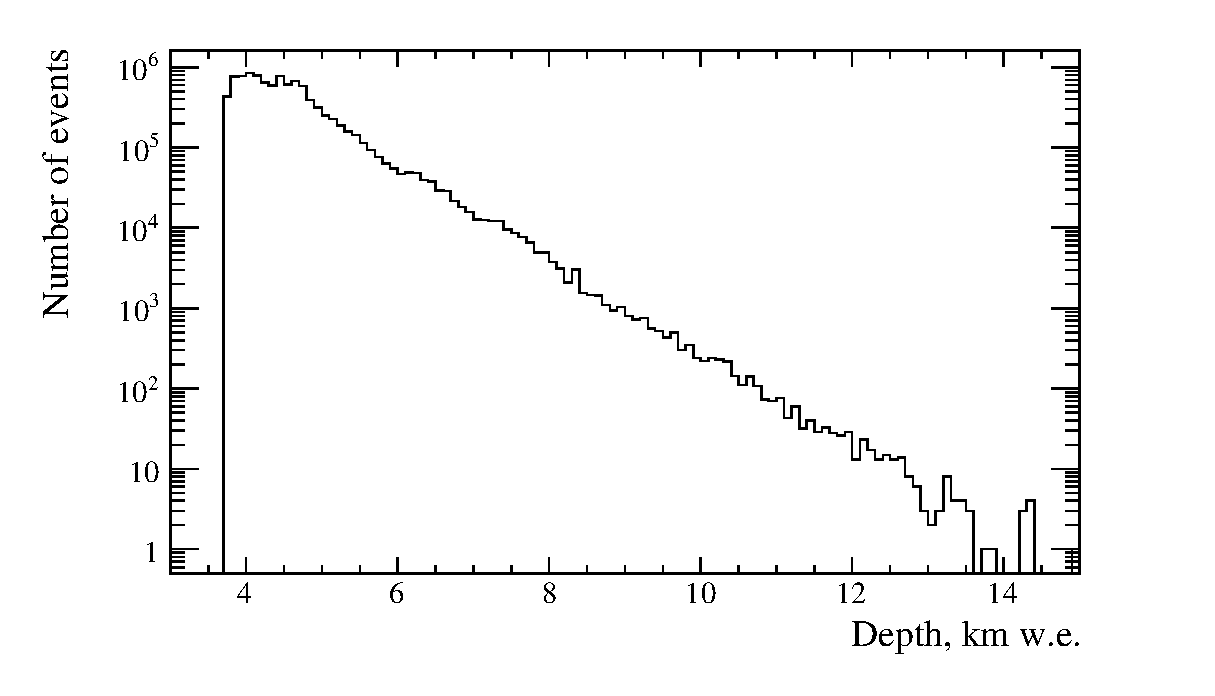
\includegraphics[width=\textwidth]{DepthCan}
    \caption{Distribution of slant depths.}
  \end{subfigure}
  \hspace{0.08\textwidth}
  \begin{subfigure}{0.45\textwidth}
    \centering
    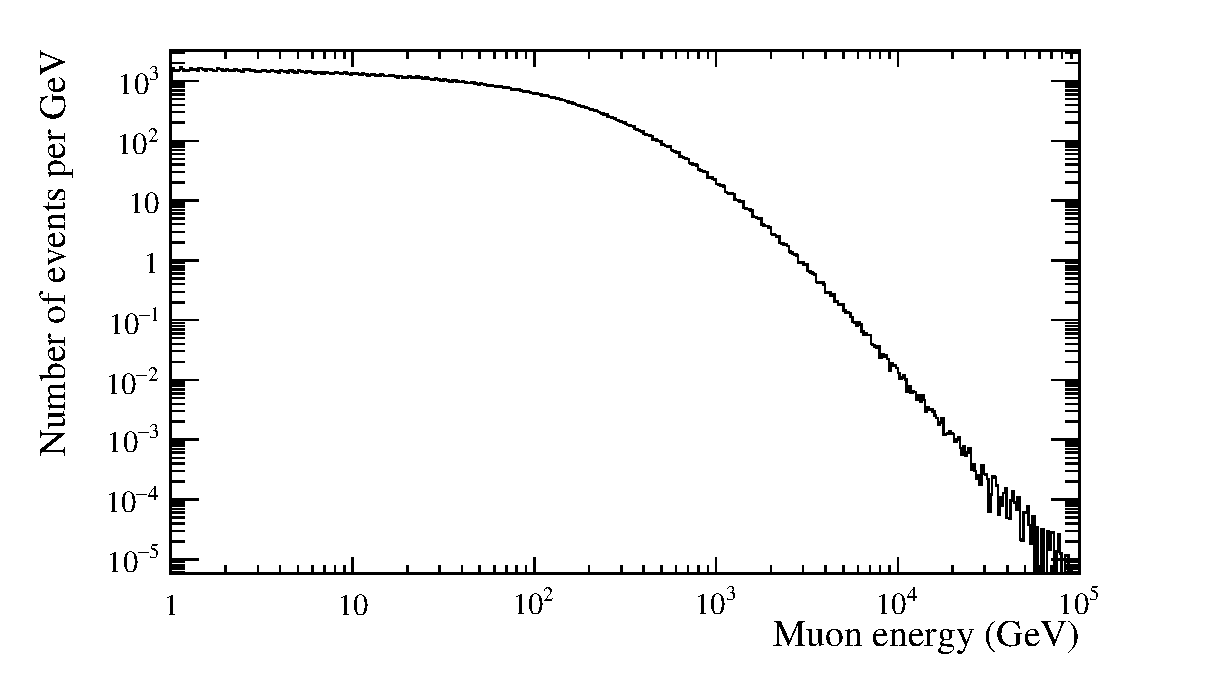
\includegraphics[width=\textwidth]{EnergyPerGeVCan}
    \caption{The energy spectrum of muon energies.}
  \end{subfigure}
  % ========
  \begin{subfigure}{0.45\textwidth}
    \centering
    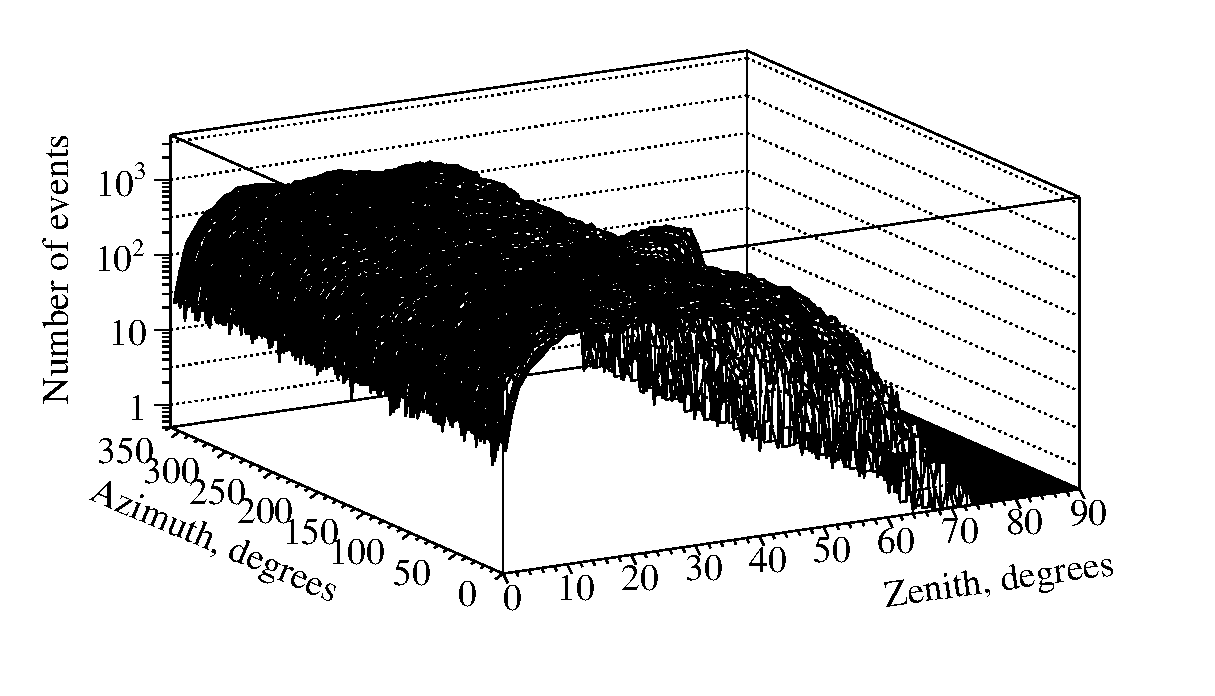
\includegraphics[width=\textwidth]{AziZenCan}
    \caption{The distribution of zenith and azimuthal angles.}
  \end{subfigure}
  \hspace{0.08\textwidth}
  \begin{subfigure}{0.45\textwidth}
    \centering
    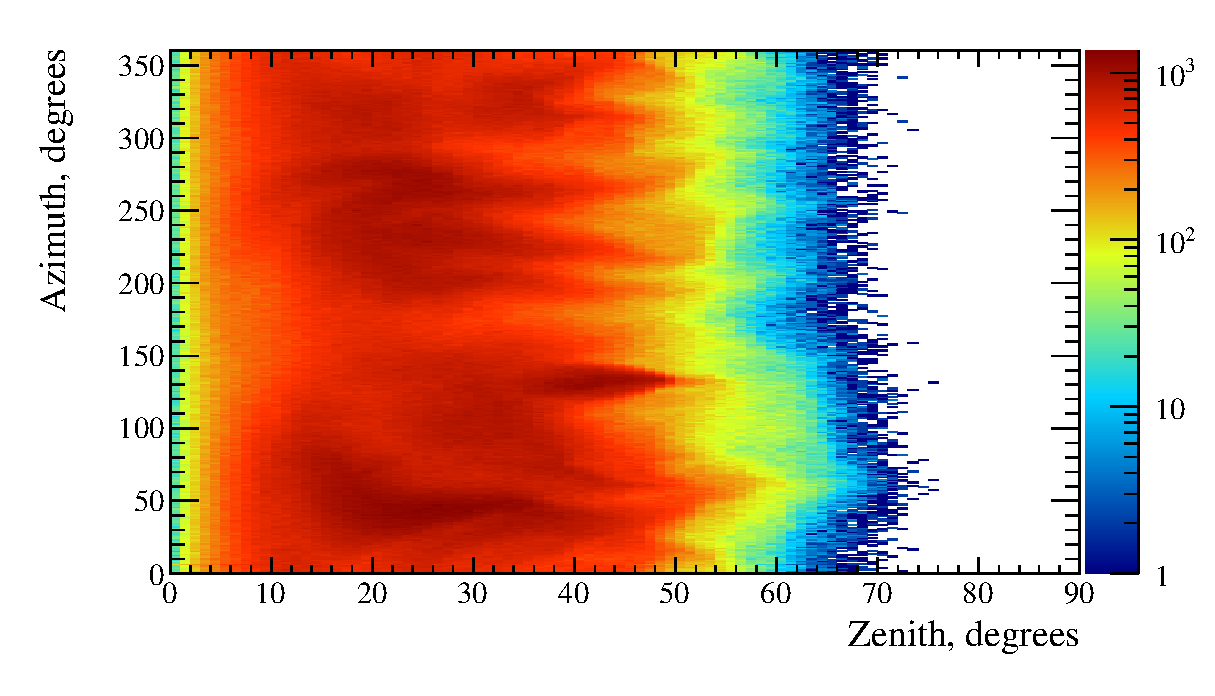
\includegraphics[width=\textwidth]{AziZenColzCan}
    \caption{The distribution of zenith and azimuthal angles, shown with a colour $z$ scale.}
  \end{subfigure}
  \caption[The distributions of some of the important quantities for muons generated by MUSUN in LArSoft]
          {The distributions of some of the important quantities for muons generated by MUSUN in LArSoft.}
  \label{fig:MUSUNIncorp}
\end{figure}

\begin{figure}[h!]
  \centering
  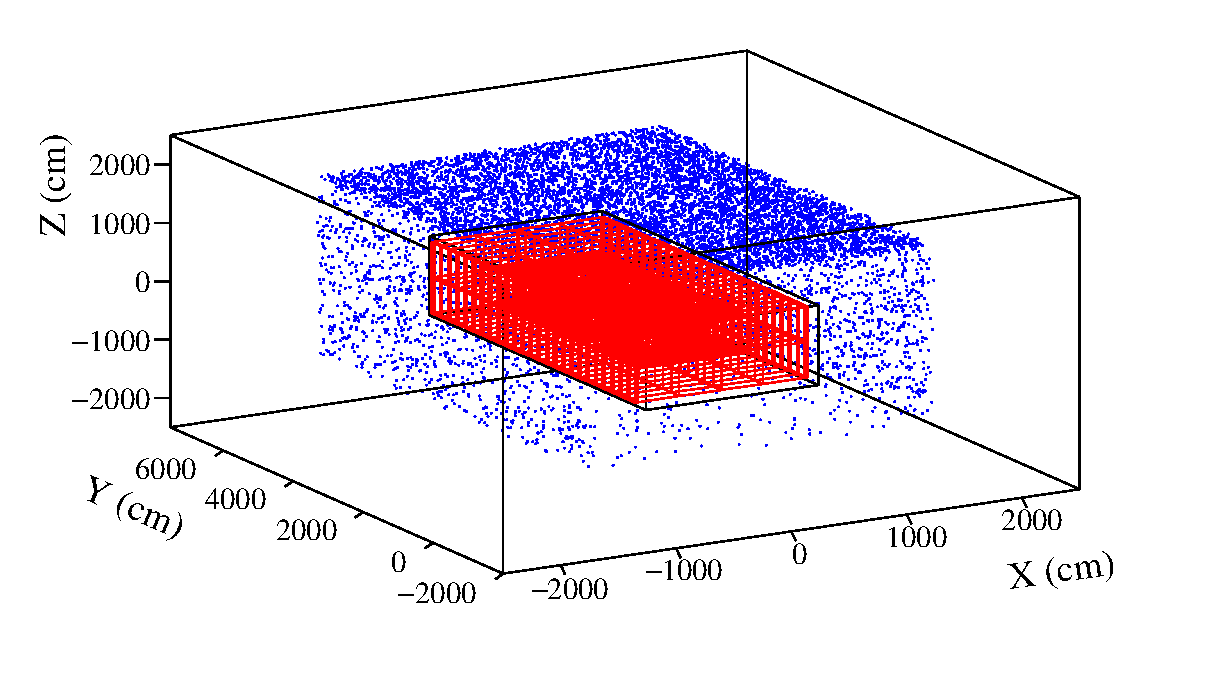
\includegraphics[width=\textwidth]{MuonPosCan}
  \caption[The initial positions of muons generated by MUSUN around a DUNE 10 kt module]
          {The initial positions of muons generated by MUSUN around a DUNE 10 kt module. The initial positions of the muons are shown as blue points, whilst the cryostat is a single black box and each TPC is a single red box.}
  \label{fig:10ktPos}
\end{figure}

It is found that the muon rate through the box upon which the muons are sampled is 0.1579 Hz, this rate is later used to normalise the background event rate in Section~\ref{sec:DUNENDK}. Of the muons that are sampled, roughly a third pass through the active volume, to give a muon rate through the active volume of 0.053 Hz. \\ 

%********************************** % Fifth Section  *************************************
\section{Cosmogenic background for nucleon decay channels in DUNE} \label{sec:DUNENDK} %Section - X.5
